\chapter{Methodology}
The research methodology focuses on developing a dynamic distance field generation system using Vulkan, a low-level
graphics API that provides precise control over GPU resources and computation. The system is designed to address the
challenges of efficient distance field generation and rendering in dynamic voxel-based environments.

\section{World Representation}
The world is stored in a GPU buffer with host and device accessibility. This design choice prioritizes flexibility in
world modification while minimizing performance overhead. Unlike traditional rendering approaches, the world buffer is
not directly rendered, which mitigates potential performance penalties associated with host-visible memory. The choice
of host-visible memory means that the host is able to update the world buffer as needed, and the updates will be visible
to the device as well, reducing complexity in staging buffers.

The world buffer will be stored in an uncompressed and dense format; this means each voxel in the world will be
present in the world buffer with all of it's associated data. In this case a voxel will be a 32-bit unsigned integer, a
value of 0 indicates an ``air'' voxel that should not be visible when rendered, while all other values indicate some
form of solid voxel.

\section{Distance Field Computation} \label{sec:df_repr}
The computation of a distance field, given a voxel grid, is the primary focus of this paper. To accomplish this a
compute shader is implemented that will output a buffer containing the discrete distance field grid for a corresponding
input voxel grid. This implementation is what will change throughout this paper as new algorithms and optimizations are
added. The distance field will contain the Manhattan distance to the nearest solid voxel, this is important for accurate
ray marching of the distance field as described in Section~\ref{sec:ray_marching}. The relation between the voxel grid,
and its corresponding discrete distance field can be seen in Figure~\ref{fig:voxel_grid_df_rel}.

\begin{figure}[htbp]
    \centering
    \begin{subfigure}{0.49\textwidth}
        \centering
        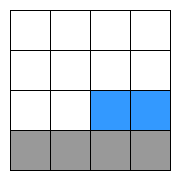
\includegraphics[width=\textwidth]{figures/voxel_grid.drawio.png}
        \caption{A 2D representation of the world. Empty voxels are indicated by white cells.}
        \label{fig:voxel_grid}
    \end{subfigure}
    \hfill
    \begin{subfigure}{0.49\textwidth}
        \centering
        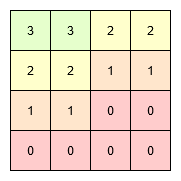
\includegraphics[width=\textwidth]{figures/voxel_grid_df.drawio.png}
        \caption{The Manhattan discrete distance field representation of the world in~\ref{fig:voxel_grid}.}
        \label{fig:voxel_grid_df}
    \end{subfigure}
    \caption{Illustration of the relation between a raw representation of a world, and its corresponding discrete
        distance field.}
    \label{fig:voxel_grid_df_rel}
\end{figure}

The computation of a distance field should not occur every frame as that would negatively impact the frame rate of an
application. Instead, the CPU will update the world state to ``dirty'' to indicate that the distance field needs to be
re-generated to reflect the newest state of the world. The workflow for this can be seen in Figure~\ref{fig:df_update_proc}

\begin{figure}[htbp]
    \centering
    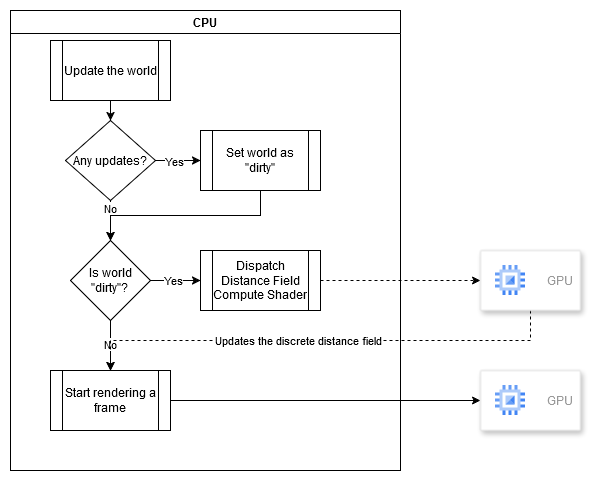
\includegraphics[width=0.8\textwidth]{figures/df_update_proc.drawio.png}
    \caption{Illustration of the computational workflow required in deciding when to update the discrete distance field
        of a world.}
    \label{fig:df_update_proc}
\end{figure}

To facilitate voxels having colors, colour information is encoded into the distance field. The distance field buffer
will be a 1-dimensional unsigned integer array. The highest 8 bits define the distance to the nearest solid voxel using
the Manhattan distance, the lowest 8 bits define the colour of the voxel in a compressed RGB332 format; voxel colours
are hard-coded into the distance field as can be seen in Figure~\ref{fig:df_repr}.

\begin{figure}[htbp]
    \centering
    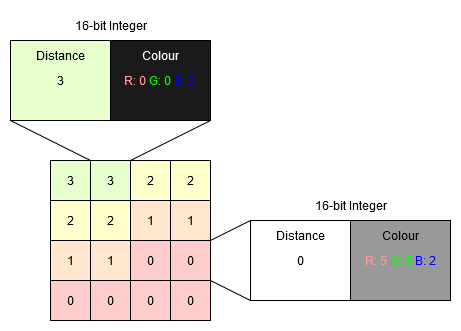
\includegraphics[width=0.8\textwidth]{figures/df_repr.drawio.png}
    \caption{Based on the same distance field as in~\ref{fig:voxel_grid_df}, the underlying integer of an empty and
        solid voxel are shown.}
    \label{fig:df_repr}
\end{figure}

\FloatBarrier

\section{Rendering and Ray Marching}\label{sec:ray_marching}
The rendering is handled by a ray marching compute shader; the distance field is the only input to this shader. The ray
marcher utilizes a digital differential analyzer to traverse through a voxel grid quickly~\cite{amanatides1987fast}.
This approach ensures a ray traversing the distance field grid will traverse each voxel along the ray, as other methods
like sphere marching could result in artifacts due to a ray ``missing'' a voxel, when using the Manhattan distance; the
steps a ray takes through the world can be seen in Figure~\ref{fig:df_dda}.

The ray marching compute shader will use a 3D perspective camera, that can move around the world. A ray can:

\begin{enumerate}
    \item Miss the world entirely, this should result in a sky color being output at that pixel.
    \item Hit the world, but not hit any solid voxels. A solid voxel is determined as a distance of 0. This will also
          result in a sky color being output at that pixel.
    \item Hit the world, and hit a solid voxel. This will result in the color at that voxel being output to the pixel.
\end{enumerate}

\begin{figure}[htbp]
    \centering
    \begin{subfigure}[t]{0.32\textwidth}
        \centering
        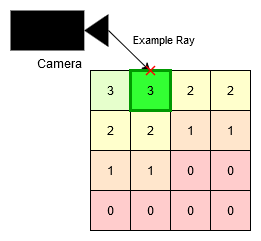
\includegraphics[width=\textwidth]{figures/df_dda_1.drawio.png}
        \caption{A ray is initially shot from the camera, hitting an outermost voxel of the world; a distance of ``3''
            is read from the distance field.}
    \end{subfigure}
    \hfill
    \begin{subfigure}[t]{0.32\textwidth}
        \centering
        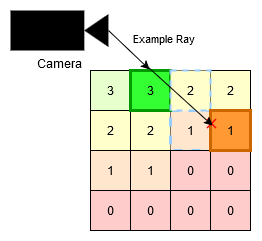
\includegraphics[width=\textwidth]{figures/df_dda_2.drawio.png}
        \caption{The ray advances 3 voxels using DDA~\protect\cite{amanatides1987fast}, before reading the distance
            field again. A distance of ``1'' is found, so the ray should continue marching through the world.}
    \end{subfigure}
    \hfill
    \begin{subfigure}[t]{0.32\textwidth}
        \centering
        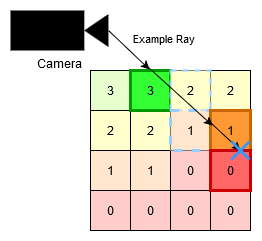
\includegraphics[width=\textwidth]{figures/df_dda_3.drawio.png}
        \caption{The ray advances the final distance, as per the previous step, finally hitting a voxel with a distance
            of ``0''. This marks the end of the ray marching, and a colour can be read from the distance field for it to
            be rendered.}
    \end{subfigure}
    \caption{Example of a ray marching through a discrete distance field using DDA~\protect\cite{amanatides1987fast}.}
    \label{fig:df_dda}
\end{figure}

\section{Demonstration Application} \label{sec:demo_app}
To demonstrate the generation of dynamic distance fields from voxel grids, a demonstration application will be
created; this application will also be used for performance testing as defined in Section~\ref{sec:perf_eval}. The
application will contain a finite voxel world that can be interacted with, voxels can be placed and deleted by the user.

The size of the world, and parameters of the distance field generation algorithm, can be altered to allow for the quick
execution of different performance tests. SVO implementations typically see upwards of 10 voxel
levels~\cite{laine2010efficient} resulting in a world size of at least 1024\textsuperscript{3}, all the way to worlds of
sizes 65536\textsuperscript{3}. The simulation will be run at different world sizes but will be limited by memory
consumption due to the uncompressed nature of the world representation and distance field.

\subsection{Vulkan Architecture}
To support the graphical demonstration application and the compute pipeline for the algorithm, the Vulkan API will be used.
Vulkan provides low-overhead, high-performance access to GPU resources, offering fine-grained control over memory
management, synchronization, and pipeline configuration. This level of control will be essential for achieving the
performance characteristics and flexibility required by the project. However, Vulkan's power comes with significant
complexity: it demands meticulous management of resources, explicit synchronization, and a steep learning curve compared
to higher-level graphics APIs such as OpenGL or DirectX 11.

Developing with Vulkan will require a substantial upfront investment in infrastructure code, but will ultimately enable
a highly efficient and predictable execution environment tailored to the specific needs of the application. To
accelerate development, the initial setup of compute pipelines and rendering was based on the
\textit{interactive fractal} example provided by the Vulkano project~\cite{vulkano-example}.

\section{Performance Evaluation}\label{sec:perf_eval}
As part of the evaluation of the distance field generation in a dynamic environment, several performance metrics need to
be gathered.

The performance test will be run multiple times with the same parameters to ensure accurate metrics are gathered; for
each implementation of the distance field computation, the demonstration application will be run using differing world
sizes, this may vary from implementation to implementation depending on their specific limitations. Results between
implementations will also be evaluated.

To ensure a consistent test environment, the demonstration application will be modified to automatically modify the
world at set intervals; this will mean that results will be reproducible when using the same seed. Voxels will be placed
and deleted from the world at random positions, with random brush sizes.

\subsection{Frame Performance Metrics}\label{sec:frame_perf_metrics}
Frame performance metrics will help in determining whether the application can run in real-time in a ``playable'' speed.
The minimum required frame rate for a game to be deemed playable is a heavily debated topic; however, player performance
typically hits a plateau above 60 frame-per-second (FPS)~\cite{claypool2007frame}, with 30 FPS being a solid starting
point. For this paper, a minimum target of 30 FPS will be set; this minimum FPS is what should be seen while the world
is being actively updated, it is expected that when no updates are being carried out the ray marching of the world should
stay above 30 FPS consistently.

The delta time of each frame will be recorded while the application is running, and the frame rate will be calculated
using the equation~\ref{eq:fps_dt}.

\begin{equation}\label{eq:fps_dt}
    \text{FPS} = \frac{1000}{\text{dt}_{\text{ms}}}
\end{equation}

Both the overall frame performance of the application, and during distance field computation, will be gathered.

\subsection{Distance Field Computation Metrics}\label{sec:distance_field_metrics}
The primary metric used here will be the execution time. Assuming a 30 FPS target, the frame time is 33.33ms, this means
for any given frame all application operations must take less than 33.33ms to achieve the target FPS; the upper
limit for distance field execution time is 33.33ms which would assume all other factors like ray marching and
presenting a frame take no time in a frame.

\break

\section{Limitations and Considerations}
The performance of the distance field computation, and the rendering, is highly hardware dependent; factors such as:

\begin{enumerate}
    \item GPU specifications
    \item Memory configuration
    \item Driver versions
\end{enumerate}

With this in mind the performance testing for this paper is carried out on a laptop with the following hardware
specifications, tests will be carried out while the laptop is plugged into a power source and all battery saving and
energy efficient modes will be disabled:

\begin{description}
    \item \textbf{\textit{CPU:}}~AMD Ryzen 9 5900HS with Radeon Graphics @ 3.3GHz
    \item \textbf{\textit{GPU:}}~NVIDIA GeForce RTX 3070 Laptop GPU
    \item \textbf{\textit{RAM:}}~16384MB @ 3200 MT/s
\end{description}
